\subsection{Resultate}

Mit dieser Arbeit wurde das cloudbasiertes Praxisrufsystem ''Praxisruf'' erweitert.
Das erweiterte Rufsystem erlaubt es, Benachrichtigungen zu Versenden und über Sprachverbindungen zu kommunizieren.
Es wurde eine native iOS App entwickelt, welche es erlaubt Praxisruf zu bedienen.
Diese App ersetzt den Mobile Client aus dem Vorgängerprojekt und unterstützt dabei alle Funktionen des alten Clients.

Mit Amazon Polly wurde ein Service für Sprachsynthese an das System angebunden.
Diese Anbindung wird verwendet, um den Inhalt empfangener Benachrichtigungen automatisch vorzulesen.
Letztlich wurde WebRTC verwendet, um eine konfigurierbare Gegensprechanlage zu implementieren.
Diese erlaubt es mit der iOS App Sprachverbindungen über das Praxisrufsystem aufzubauen.
Sowohl das Vorlesen von Benachrichtigungen, als auch die Gegensprechanlage sind über eine Weboberfläche konfigurierbar.

Die zu Projektbeginn definierten Meilensteine M01 bis M08 wurden erreicht.
Die Funktionalen Anforderungen an das System wurden umgesetzt.
Die bestehende Infrastruktur aus dem Vorgängerprojekt wurde für dieses Projekt uneingeschränkt übernommen.
Die Komponenten Cloudservice, Messaging Service sowie Admin UI aus dem Vorgängerprojekt wurden weiterverwendet und erweitert.
Umgesetzt wurden die Meilensteine mit folgenden User Stories:

\begin{itemize}
    \item U01 - Migration bestehender Funktion im Mobile Client
    \item U02 - Benachrichtigungen vorlesen
    \item U03 - Vorlesen von Benachrichtigungen deaktivieren
    \item U04 - Button für Sprachverbindung 1:1
    \item U05 - Button für Sprachverbindung 1:n
    \item U06 - Über Sprachverbindung in Echtzeit kommunizieren
    \item U07 - Nur relevante Buttons für Sprachverbindungen anzeigen
    \item U08 - Benachrichtigungston für eingehende Sprachverbindungen
    \item U09 - Empfangene und verpasste Sprachverbindungen in Inbox anzeigen
    \item U10 - Eingehende Sprachverbindungen automatisch öffnen
    \item U11 - Sprachverbindung beenden
    \item U13 - Vorlesen von Benachrichtigungen konfigurieren
    \item U14 - Buttons für Sprachverbindungen konfigurieren
    \item U15 - Konfiguration über Admin UI vornehmen
    \item U16 - Bestehende Infrastruktur übernehmen
    \item U17 - Weiterverwendung bestehender Komponenten
    \item U18 - Native iOS Applikation
    \item U19 - Für Externe Services Amazon Webservices verwenden
\end{itemize}

Der zu Beginn definierte Projektplan konnte grösstenteils eingehalten werden.
Setup- und Konzept-Phase wurden im geplanten Zeitraum abgeschlossen.
Während der Umsetzung ist es hingegen zu mehreren Verzögerungen gekommen.
Die Umsetzung und Testen der Gegensprechanlage hat deutlich mehr Zeit beansprucht, als eingeplant wurde.
Insbesondere die Integration und effiziente Verwendung von WebRTC im nativen iOS Client war anspruchsvoller als erwartet.
Dies ist einerseits auf mangelhafte Dokumentation der verwendeten Bibliotheken zurückzuführen.
Andererseits wurde schlicht zu wenig Puffer für die Implementation und unerwartete Probleme eingeplant.
Die Verzögerungen während der Umsetzung hat dazu geführt, dass weniger Zeit als geplant für Polishing und Erweiterungen aufgewendet werden konnten.
Dementsprechend konnte der Meilenstein M09 nicht vollständig erreicht werden.
Das entwickelte System hat in den Bereichen Stabilität und Benutzerfreundlichkeit noch Lücken.

Der Meilenstein M10 betrifft Abschluss und Abgabe des Projektberichts und Entwicklung des Systems.
Er ist mit dem Abschluss dieses Projektes erfüllt.

\subsubsection{Native iOS Applikation}

Dieses Kapitel beschreibt das umgesetzte Praxisrufsystem anhand der Ansichten der iOS Applikation.
Sämtliche in diesem Kapitel dargestellten Ansichten wurden als Screenshots auf einem iPad 9.\ Generation erstellt.

\subsubsection*{Anmeldung und Konfiguration}

Der Mobile Client bietet eine einfaches Verfahren zur Anmeldung und Konfiguration.
In einem ersten Schritt gibt der Praxismitarbeitende in der Login-Ansicht Benutzername und Passwort ein (Abbildung 8.1).
Anschliessend kann er auf einer zweiten Ansicht, die gewünschte Zimmerkonfiguration wählen (Abbildung 8.2).
Benutzer, Passwort und die gewählte Konfiguration werden dabei auf dem Gerät gespeichert.
Bis sich der Benutzer manuell abmeldet, erfolgt die Anmeldung bei allen zukünftigen Starts der App automatisch.
Dabei wird die gespeicherte Kombination von Benutzer und Konfiguration wiederverwendet.

\begin{figure}[h]
    \centering
    \begin{minipage}[b]{0.45\textwidth}
        \fbox{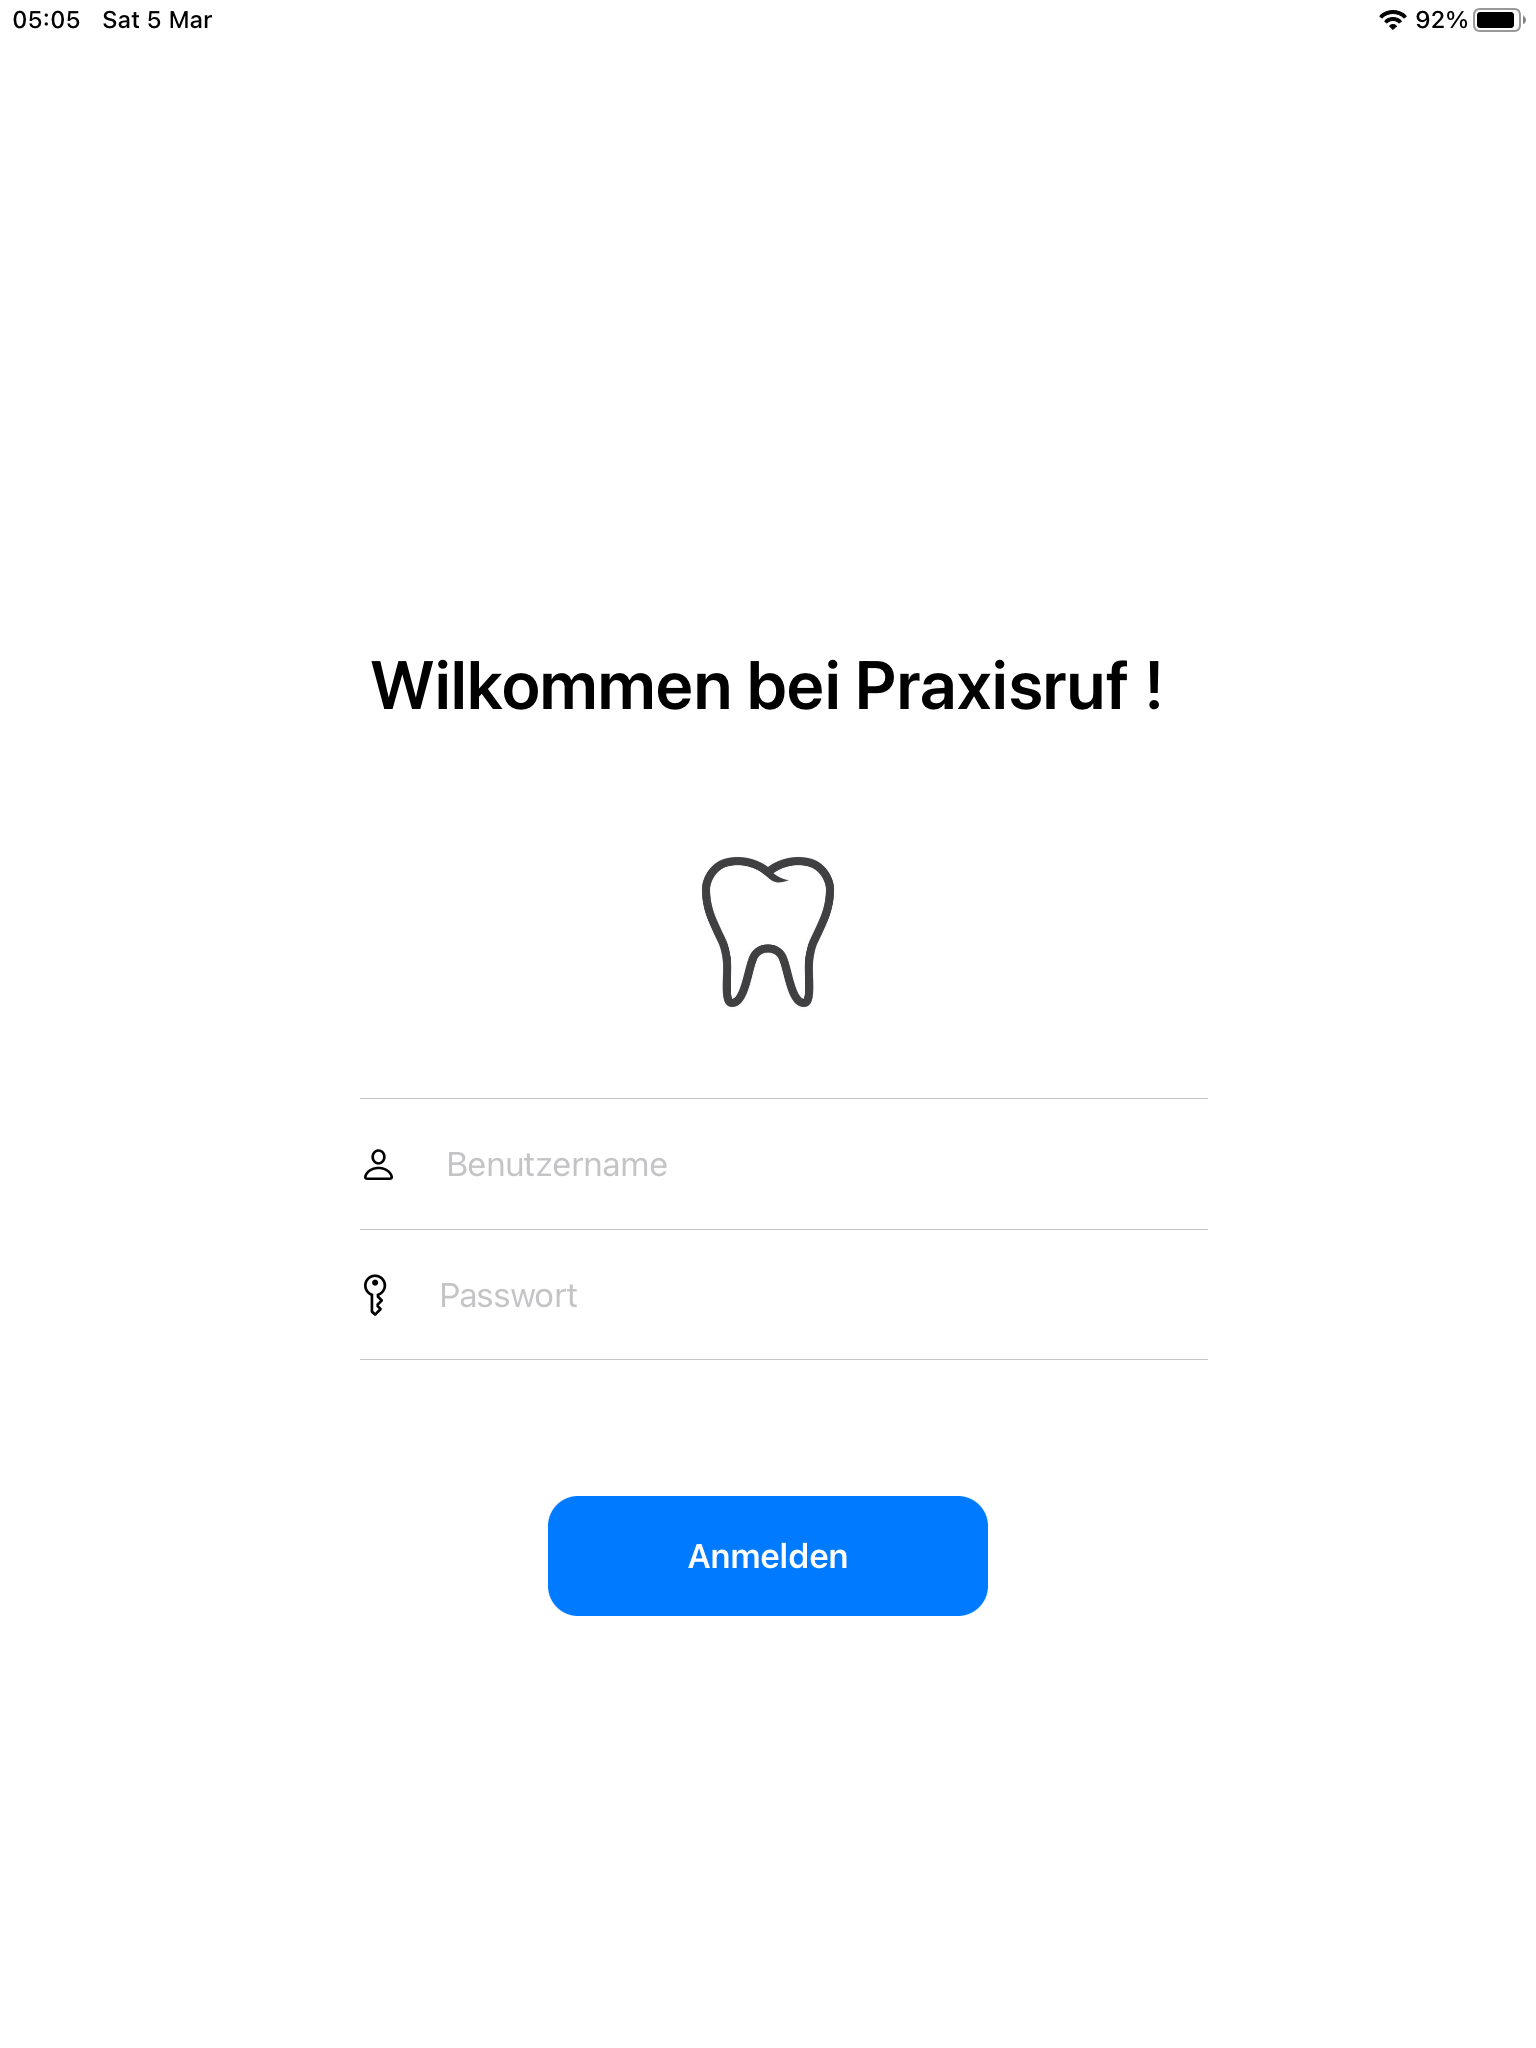
\includegraphics[width=\textwidth]{graphics/screenshots/app/login}}
        \caption{Ansicht Login}
    \end{minipage}
    \hfill
    \begin{minipage}[b]{0.45\textwidth}
        \fbox{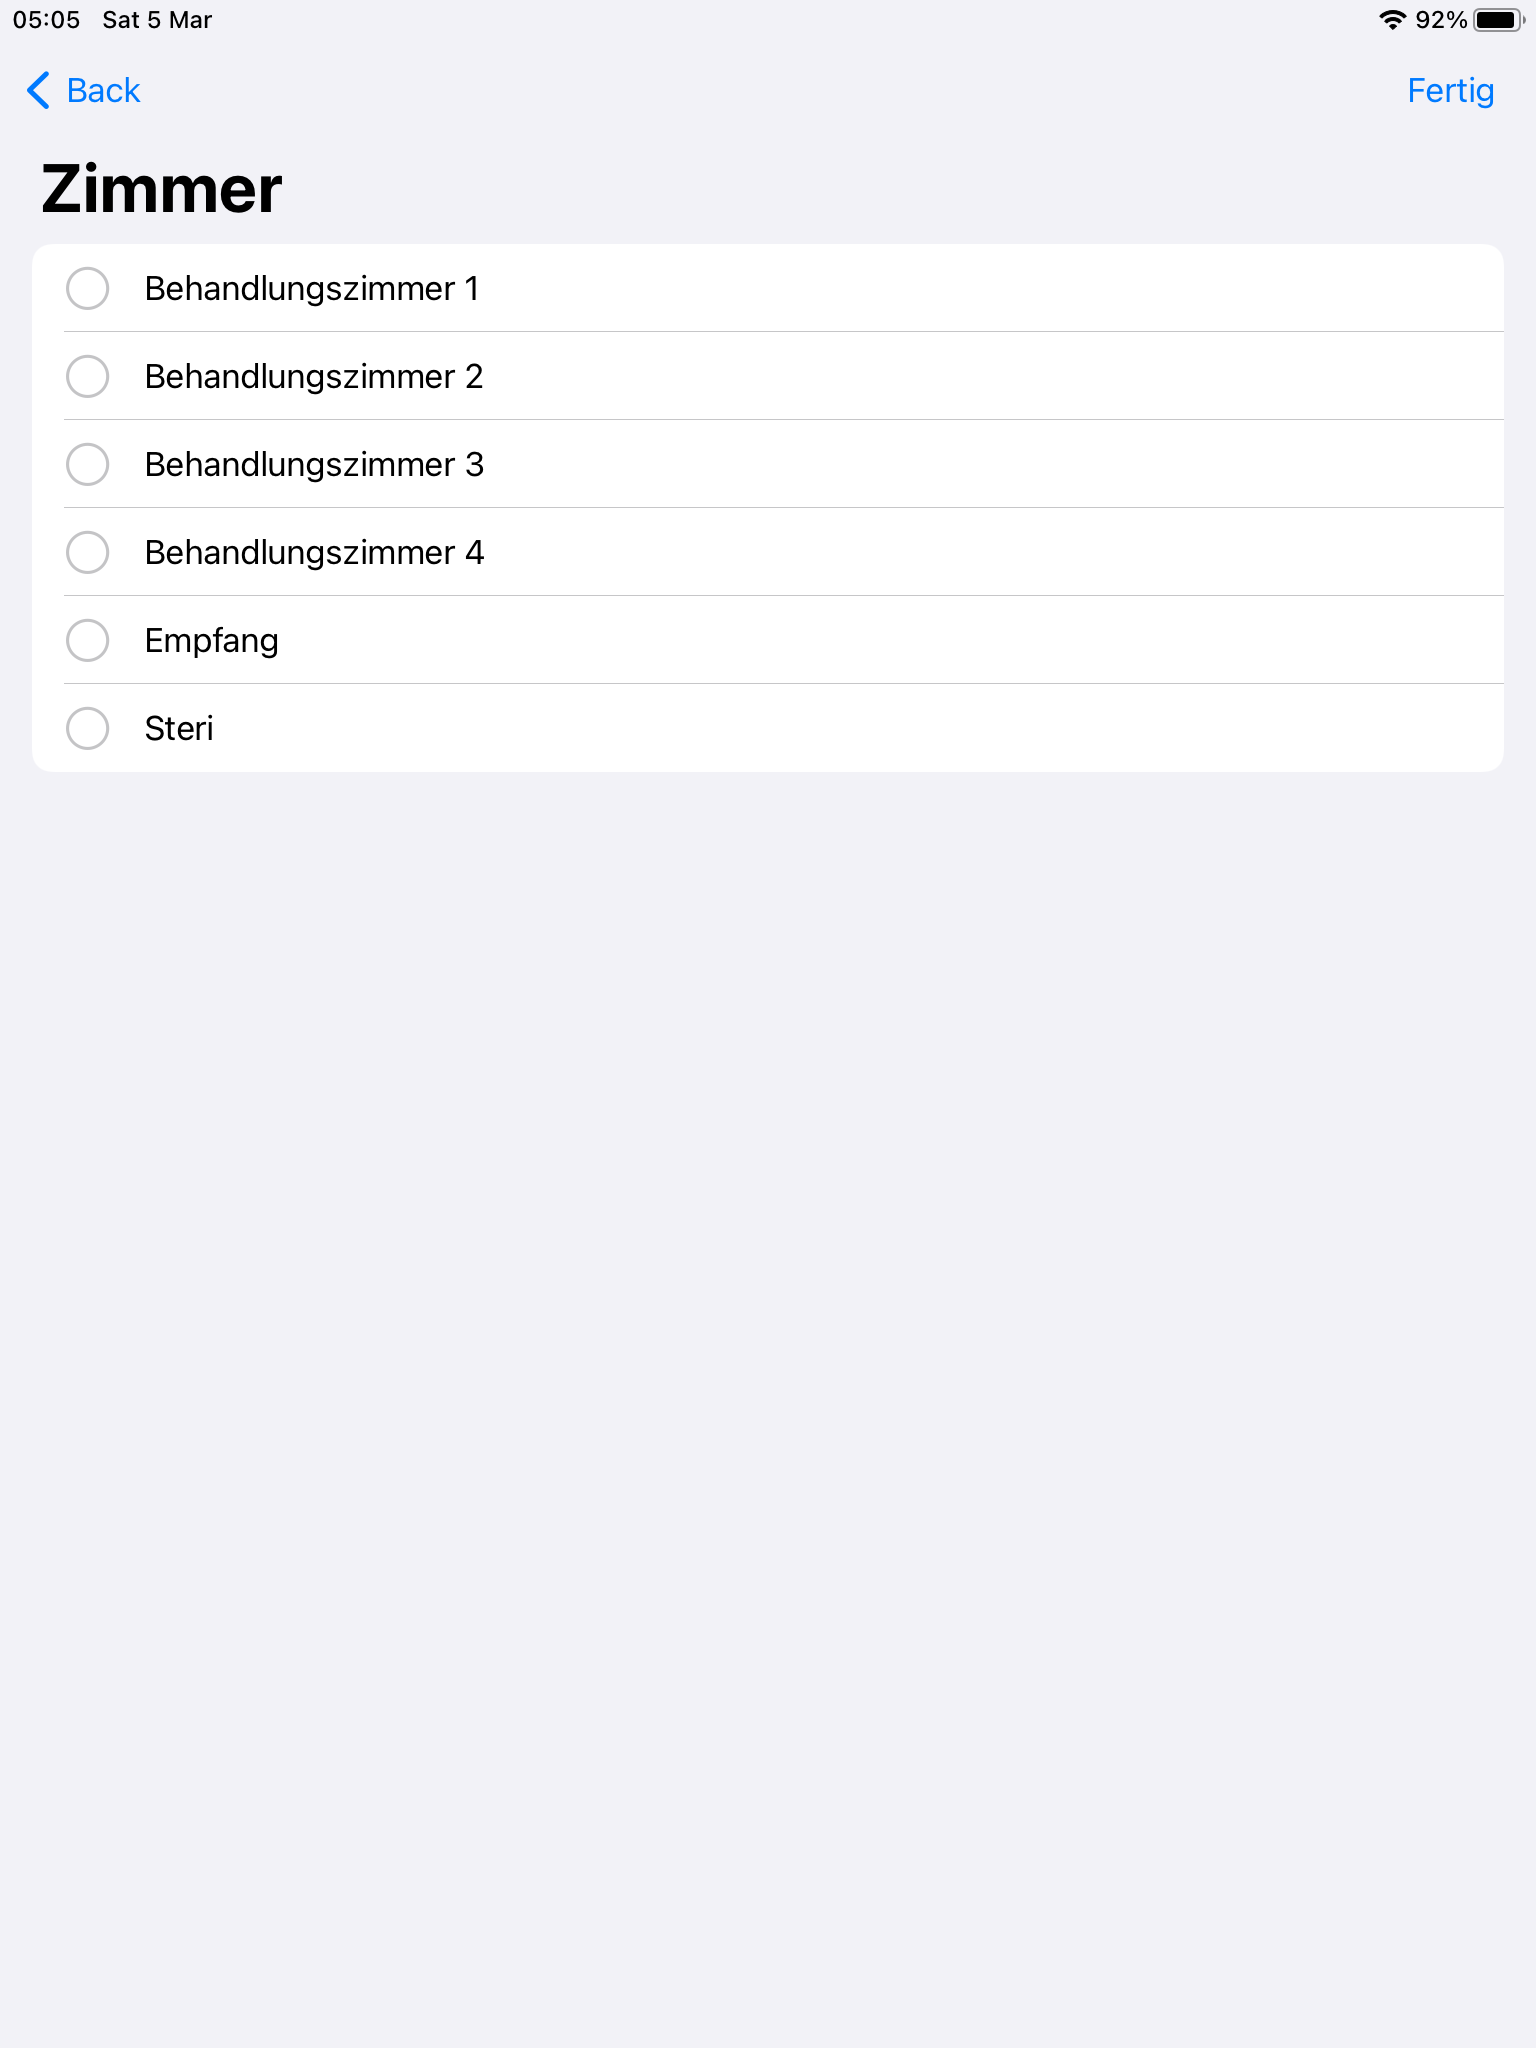
\includegraphics[width=\textwidth]{graphics/screenshots/app/client_select}}
        \caption{Ansicht Zimmerwahl }
    \end{minipage}

    \label{fig:MobileClient-Screens1}

\end{figure}

\clearpage

\subsubsection*{Startseite und Inbox}

Nach der Anmeldung und Konfigurationsauswahl wird der Benutzer auf die Hauptansicht der App weitergeleitet.
Über eine Navigationsleiste am unteren Bildschirmrand kann zwischen den Bereichen Home, Inbox und Einstellungen navigiert werden.
Der Bereich Home (Abbildung 8.3) ist in zwei Teile gegliedert.
Diese beinhalten Buttons, über welche Benachrichtigungen versendet und Sprachverbindungen gestartet werden können.
Welche Buttons zur Verfügung stehen werden durch die gewählte Zimmerkonfiguration vorgegeben und wurden im Vorfeld von Praxisadministrierenden konfiguriert.
Der Bereich Inbox (Abbildung 8.4) zeigt eine Liste von empfangenen Benachrichtigungen sowie verpassten und vergangenen Anrufen.
Einzelne Einträge in dieser Liste können durch eine Wischgeste (Swipe left) quittiert und damit entfernt werden.
Weiter können mit der Schaltfläche ''Inbox leeren'' am unteren Ende der Liste alle Einträge gleichzeitig quittiert werden.
Das quittieren von Inboxelementen geschieht ausschliesslich lokal auf dem Gerät des Empfängers.
Der Sender von Benachrichtigungen wird nicht über die Quittierung informiert.
Damit wurde das Quittieren von Elementen analog zum Vorgängerprojekt umgesetzt.

\begin{figure}[h]
    \centering
    \begin{minipage}[b]{0.45\textwidth}
        \fbox{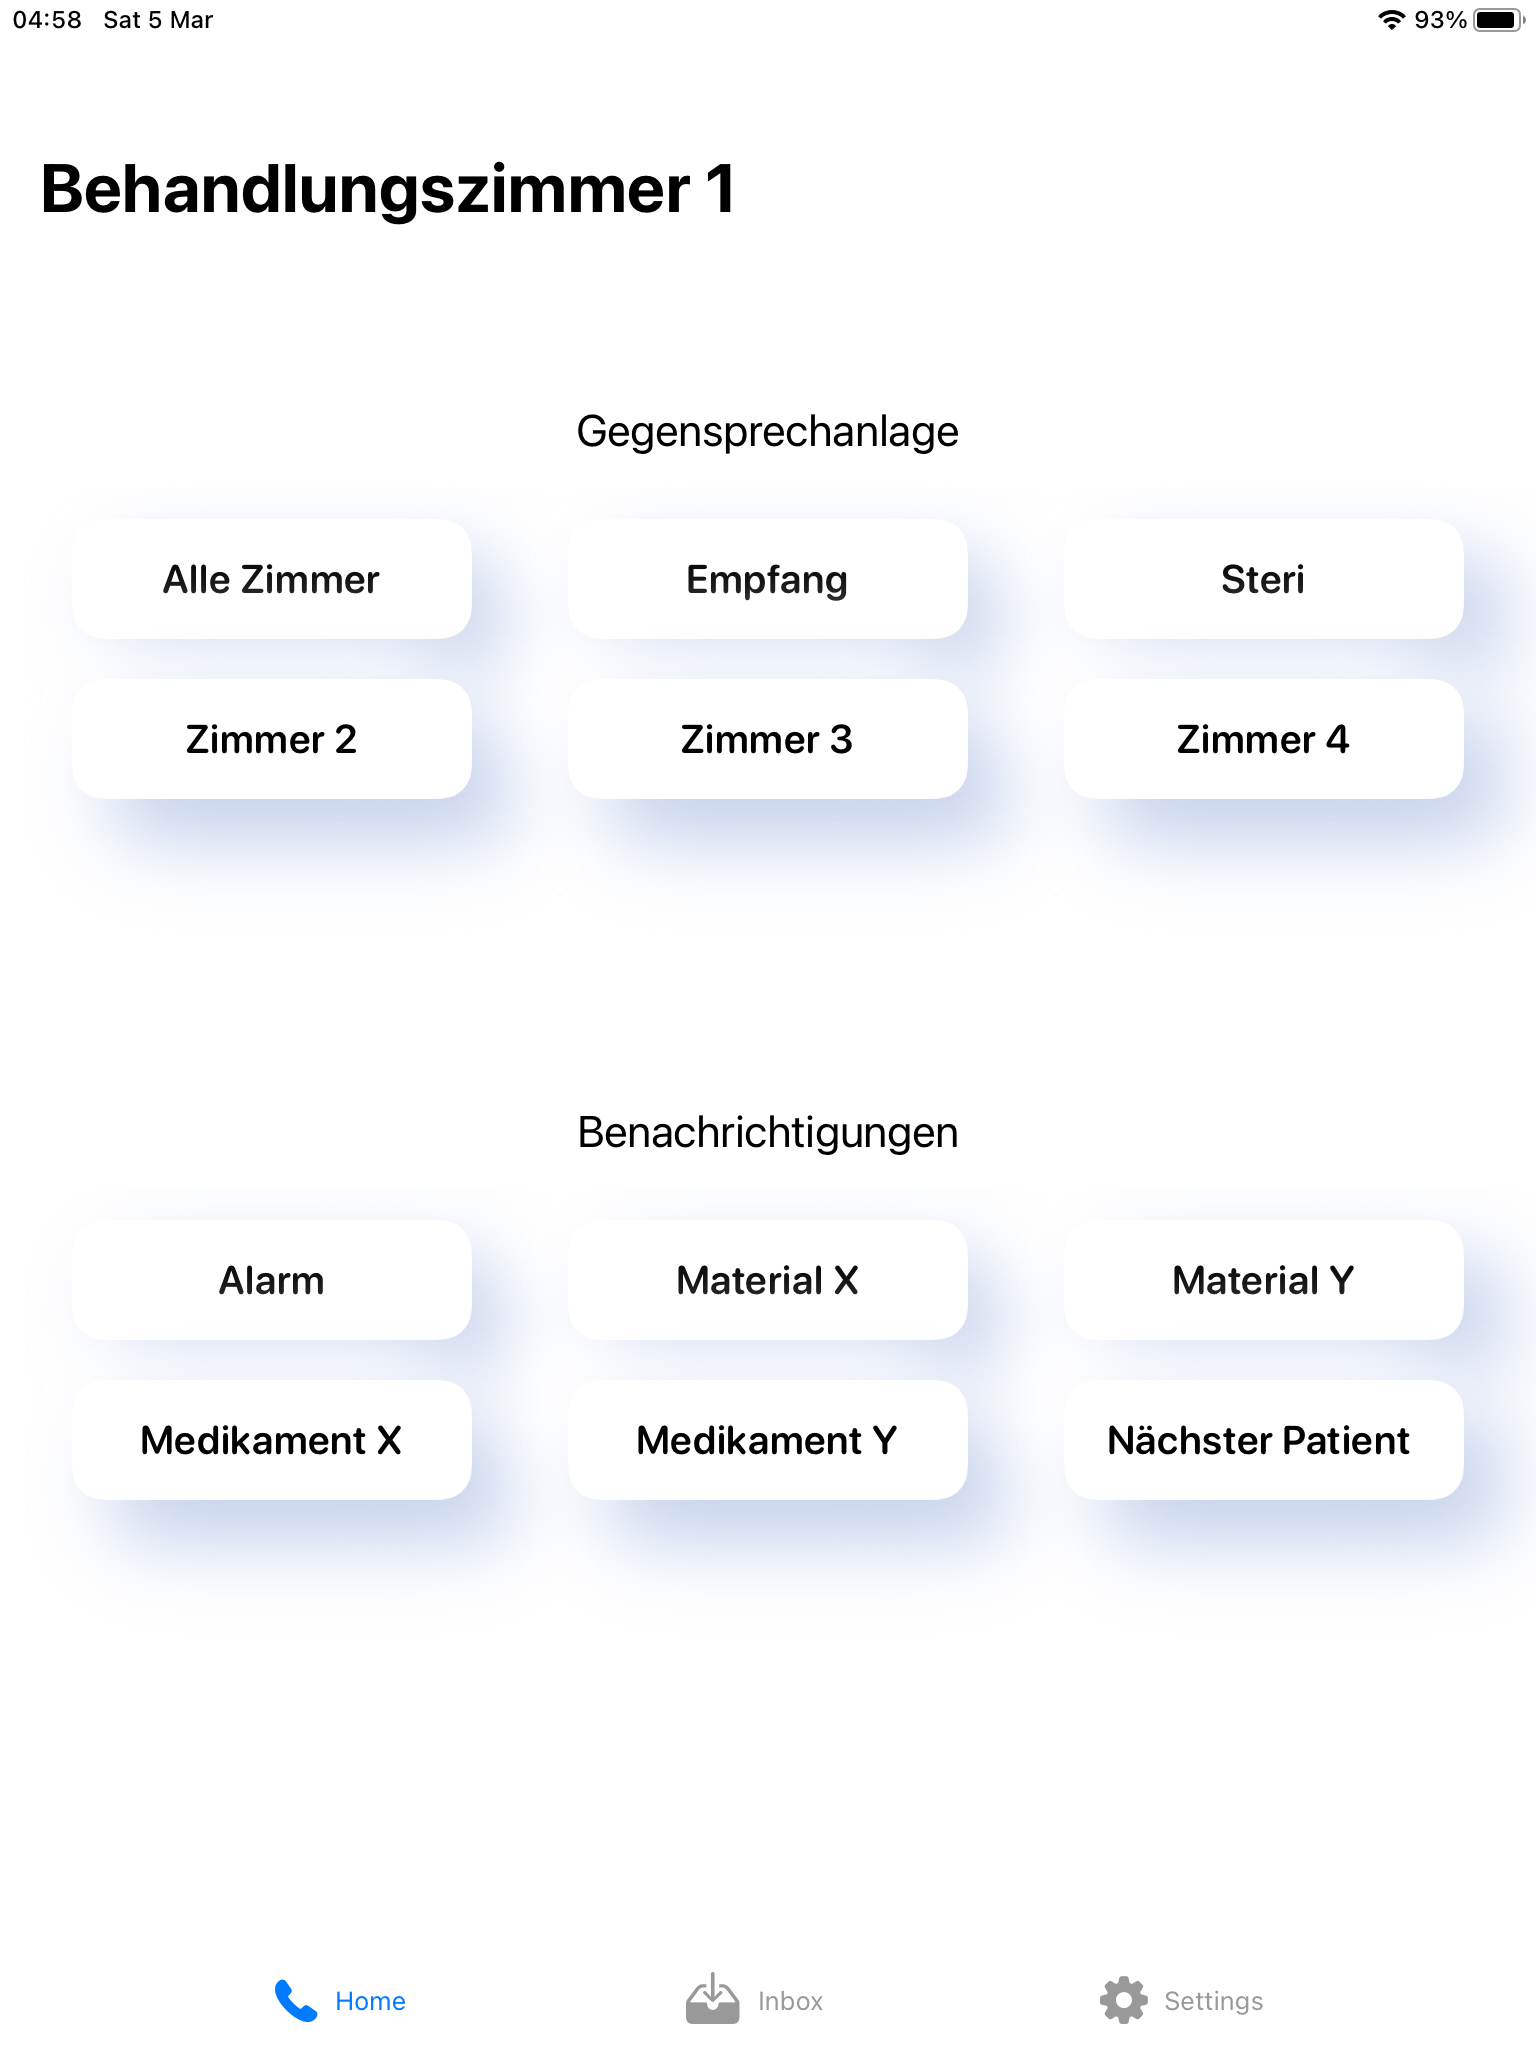
\includegraphics[width=\textwidth]{graphics/screenshots/app/home}}
        \caption{Ansicht Home}
    \end{minipage}
    \hfill
    \begin{minipage}[b]{0.45\textwidth}
        \fbox{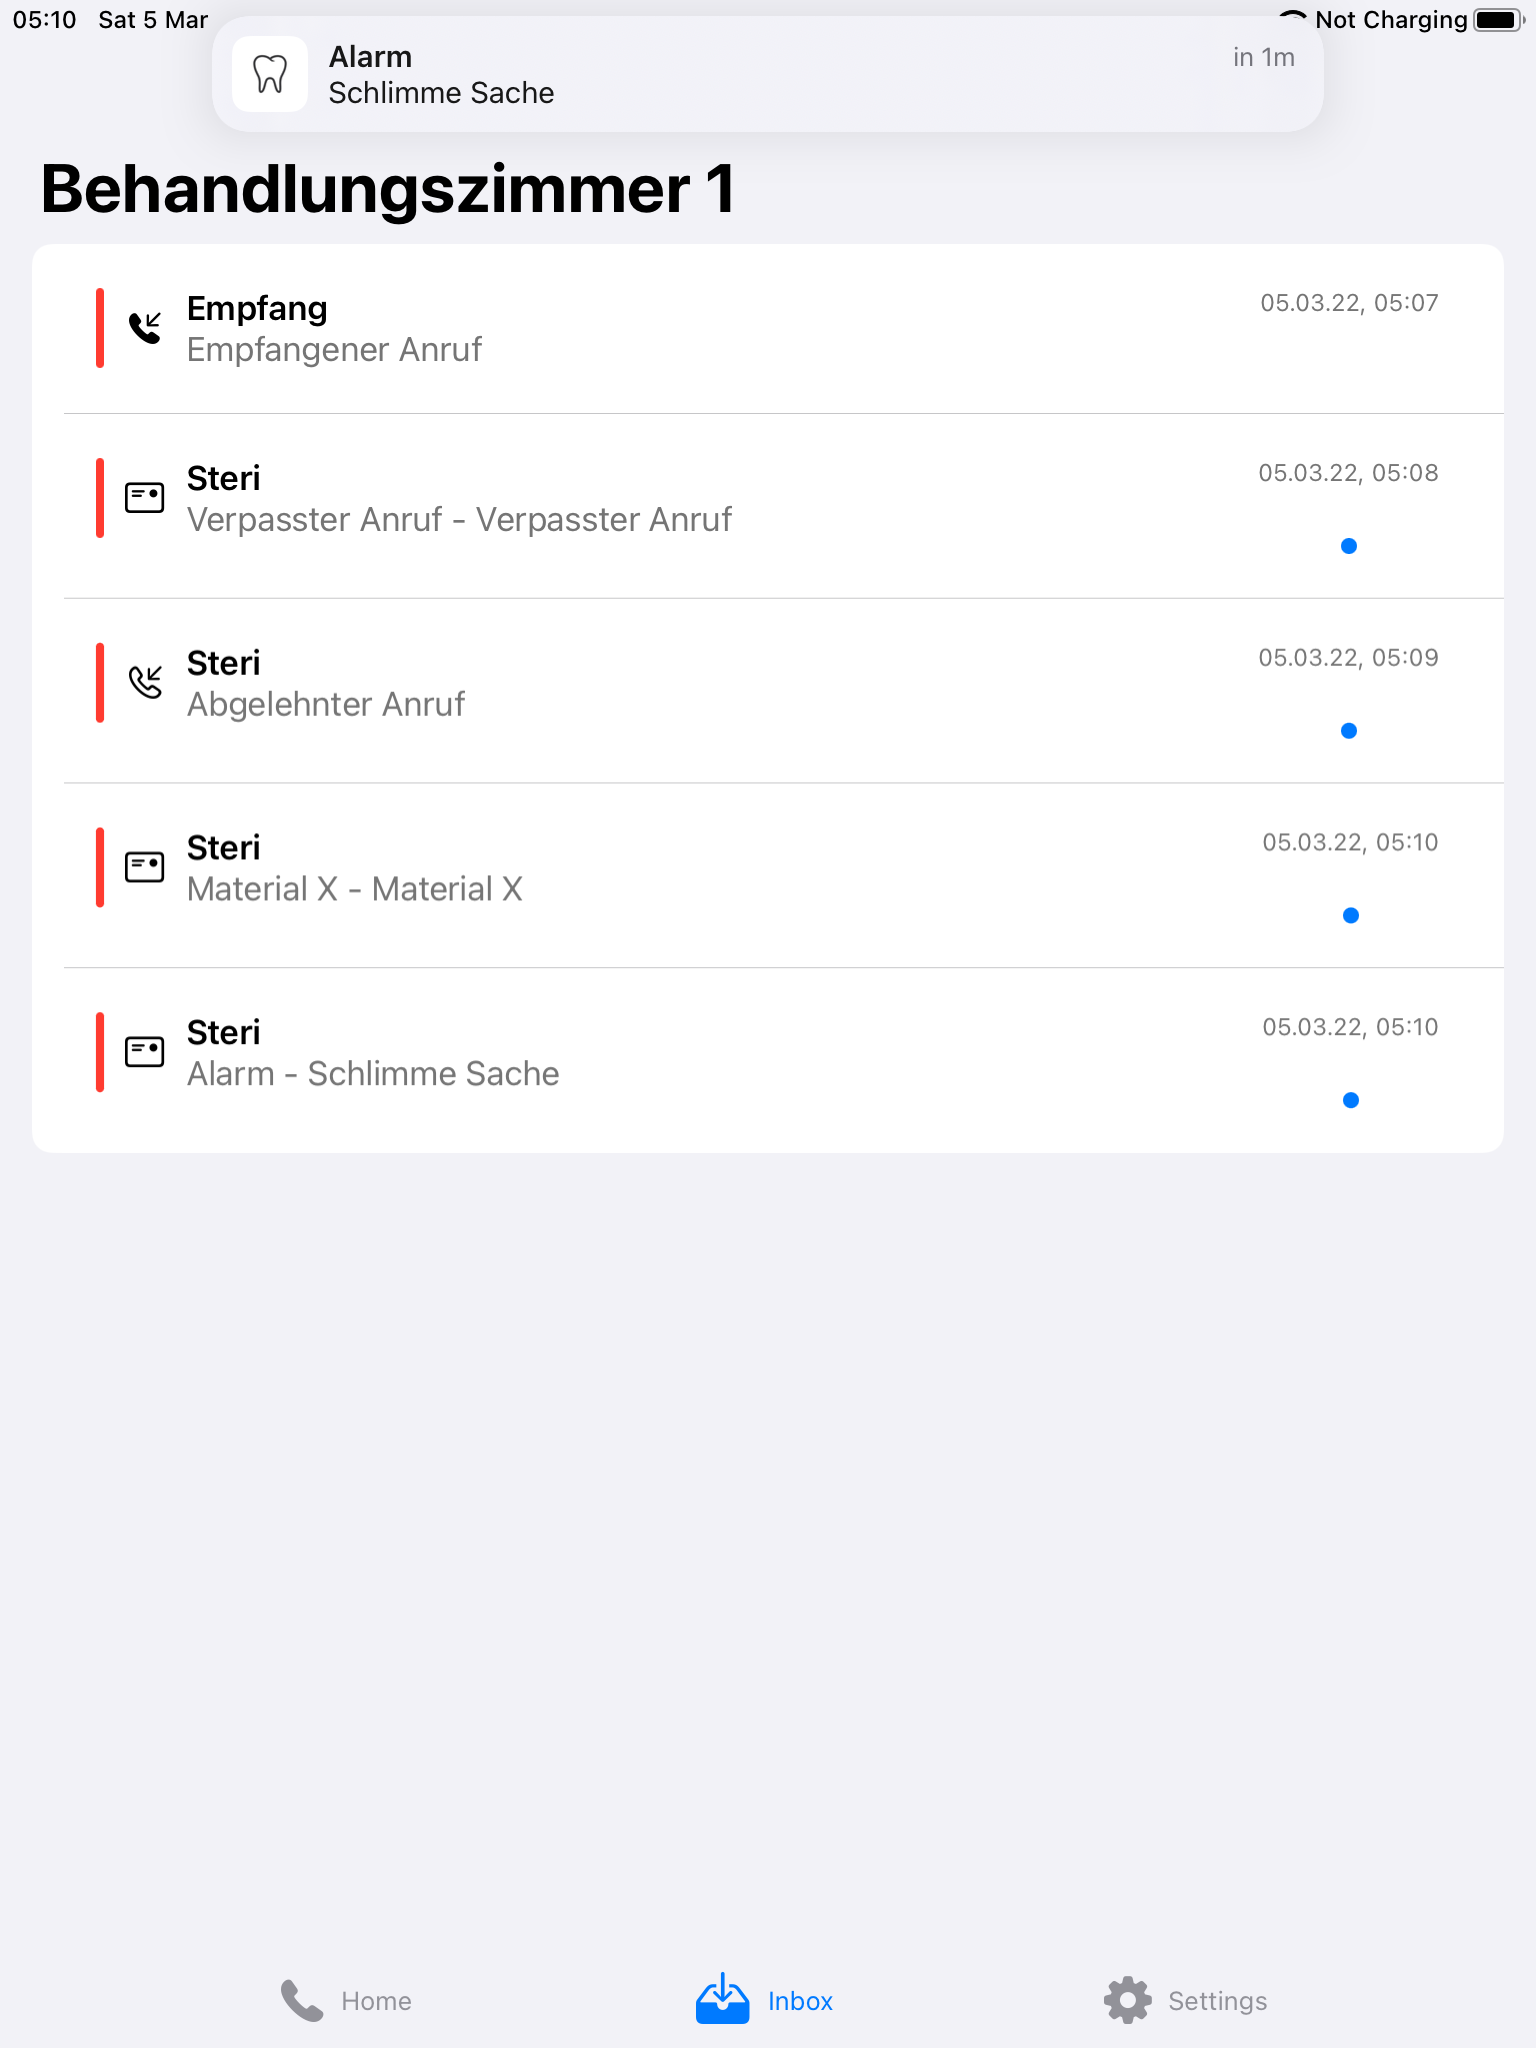
\includegraphics[width=\textwidth]{graphics/screenshots/app/inbox_alarm}}
        \caption{Ansicht Inbox}
    \end{minipage}
    \label{fig:MobileClient-Screens2}
\end{figure}

Ein Hintergrundprozess prüft in regelmässigen Abständen, ob es unquittierte Elemente in der Inbox gibt.
Ist dies der Fall wird eine Push-Benachrichtigung angezeigt und der Benachrichtigungston abgespielt.
Diese Benachrichtigung ist in Abbildung 8.4 zu sehen.
Eine Ausnahme bilden Elemente für eingehende Anrufe, die erfolgreich empfangen wurden.
Diese werden in der Inbox angezeigt und können quittiert werden.
Sie werden aber bei der Prüfung auf nicht quittierte Elemente ignoriert.

\clearpage

\subsubsection*{Einstellungen und Aktive Anrufe}

Im Bereich Einstellungen (Abbildung 8.5) werden Informationen zur gewählten Zimmerkonfiguration und dem angemeldeten Benutzer angezeigt.
Weiter können lokale Einstellungen vorgenommen werden.
Das Vorlesen von empfangenen Benachrichtigungen sowie das Empfangen von Anrufen kann hier deaktiviert werden.
Ist das Vorlesen von Benachrichtigungen deaktiviert, wird der Inhalt von Benachrichtigungen nie vorgelesen.
Benachrichtigungen können aber weiterhin empfangen und versendet werden.
Ist der Empfang von Anrufen deaktiviert, werden alle eingehenden Anrufe automatisch abgelehnt.
Dem Empfänger wird dabei eine Benachrichtigung angezeigt, die über den verpassten Anruf informiert.
Der Anrufer wird über eine Signalmeldung informiert, dass die Verbindung nicht hergestellt werden konnte.
Der Status des Empfängers wird in der Ansicht für Aktive Anrufe auf Senderseite entsprechend dargestellt.
Über einen Button kann der Benutzer sich zudem von der App abmelden.

\begin{figure}[h]
    \centering
    \begin{minipage}[b]{0.45\textwidth}
        \fbox{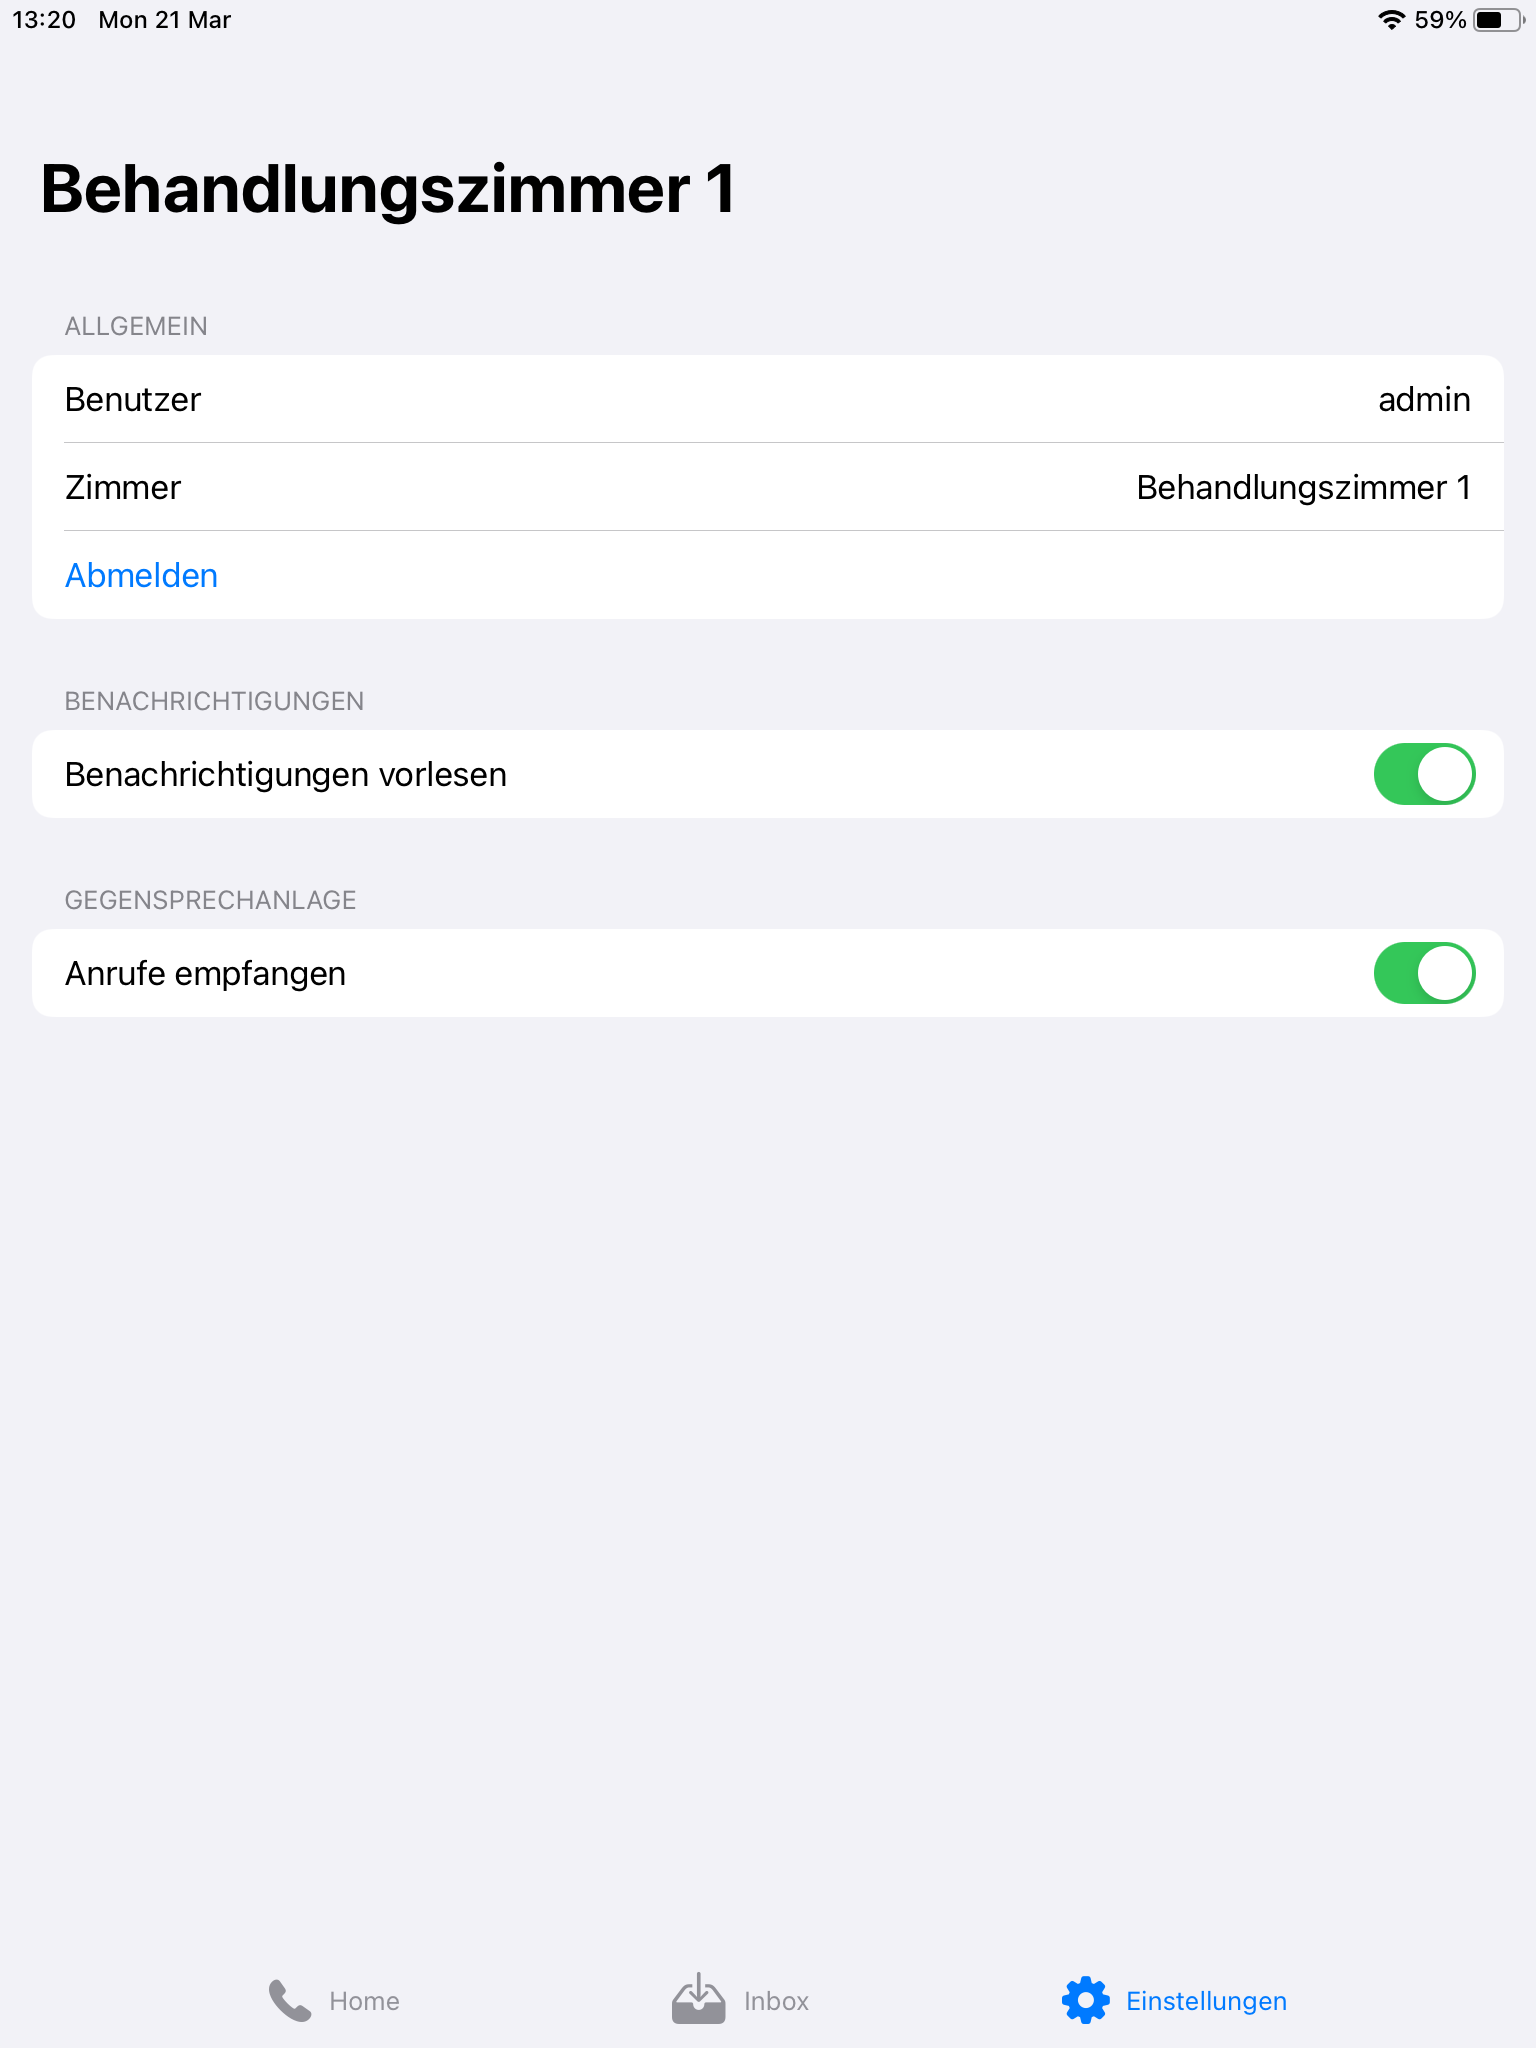
\includegraphics[width=\textwidth]{graphics/screenshots/app/settings}}
        \caption{Ansicht Einstellungen}
    \end{minipage}
    \hfill
    \begin{minipage}[b]{0.45\textwidth}
        \fbox{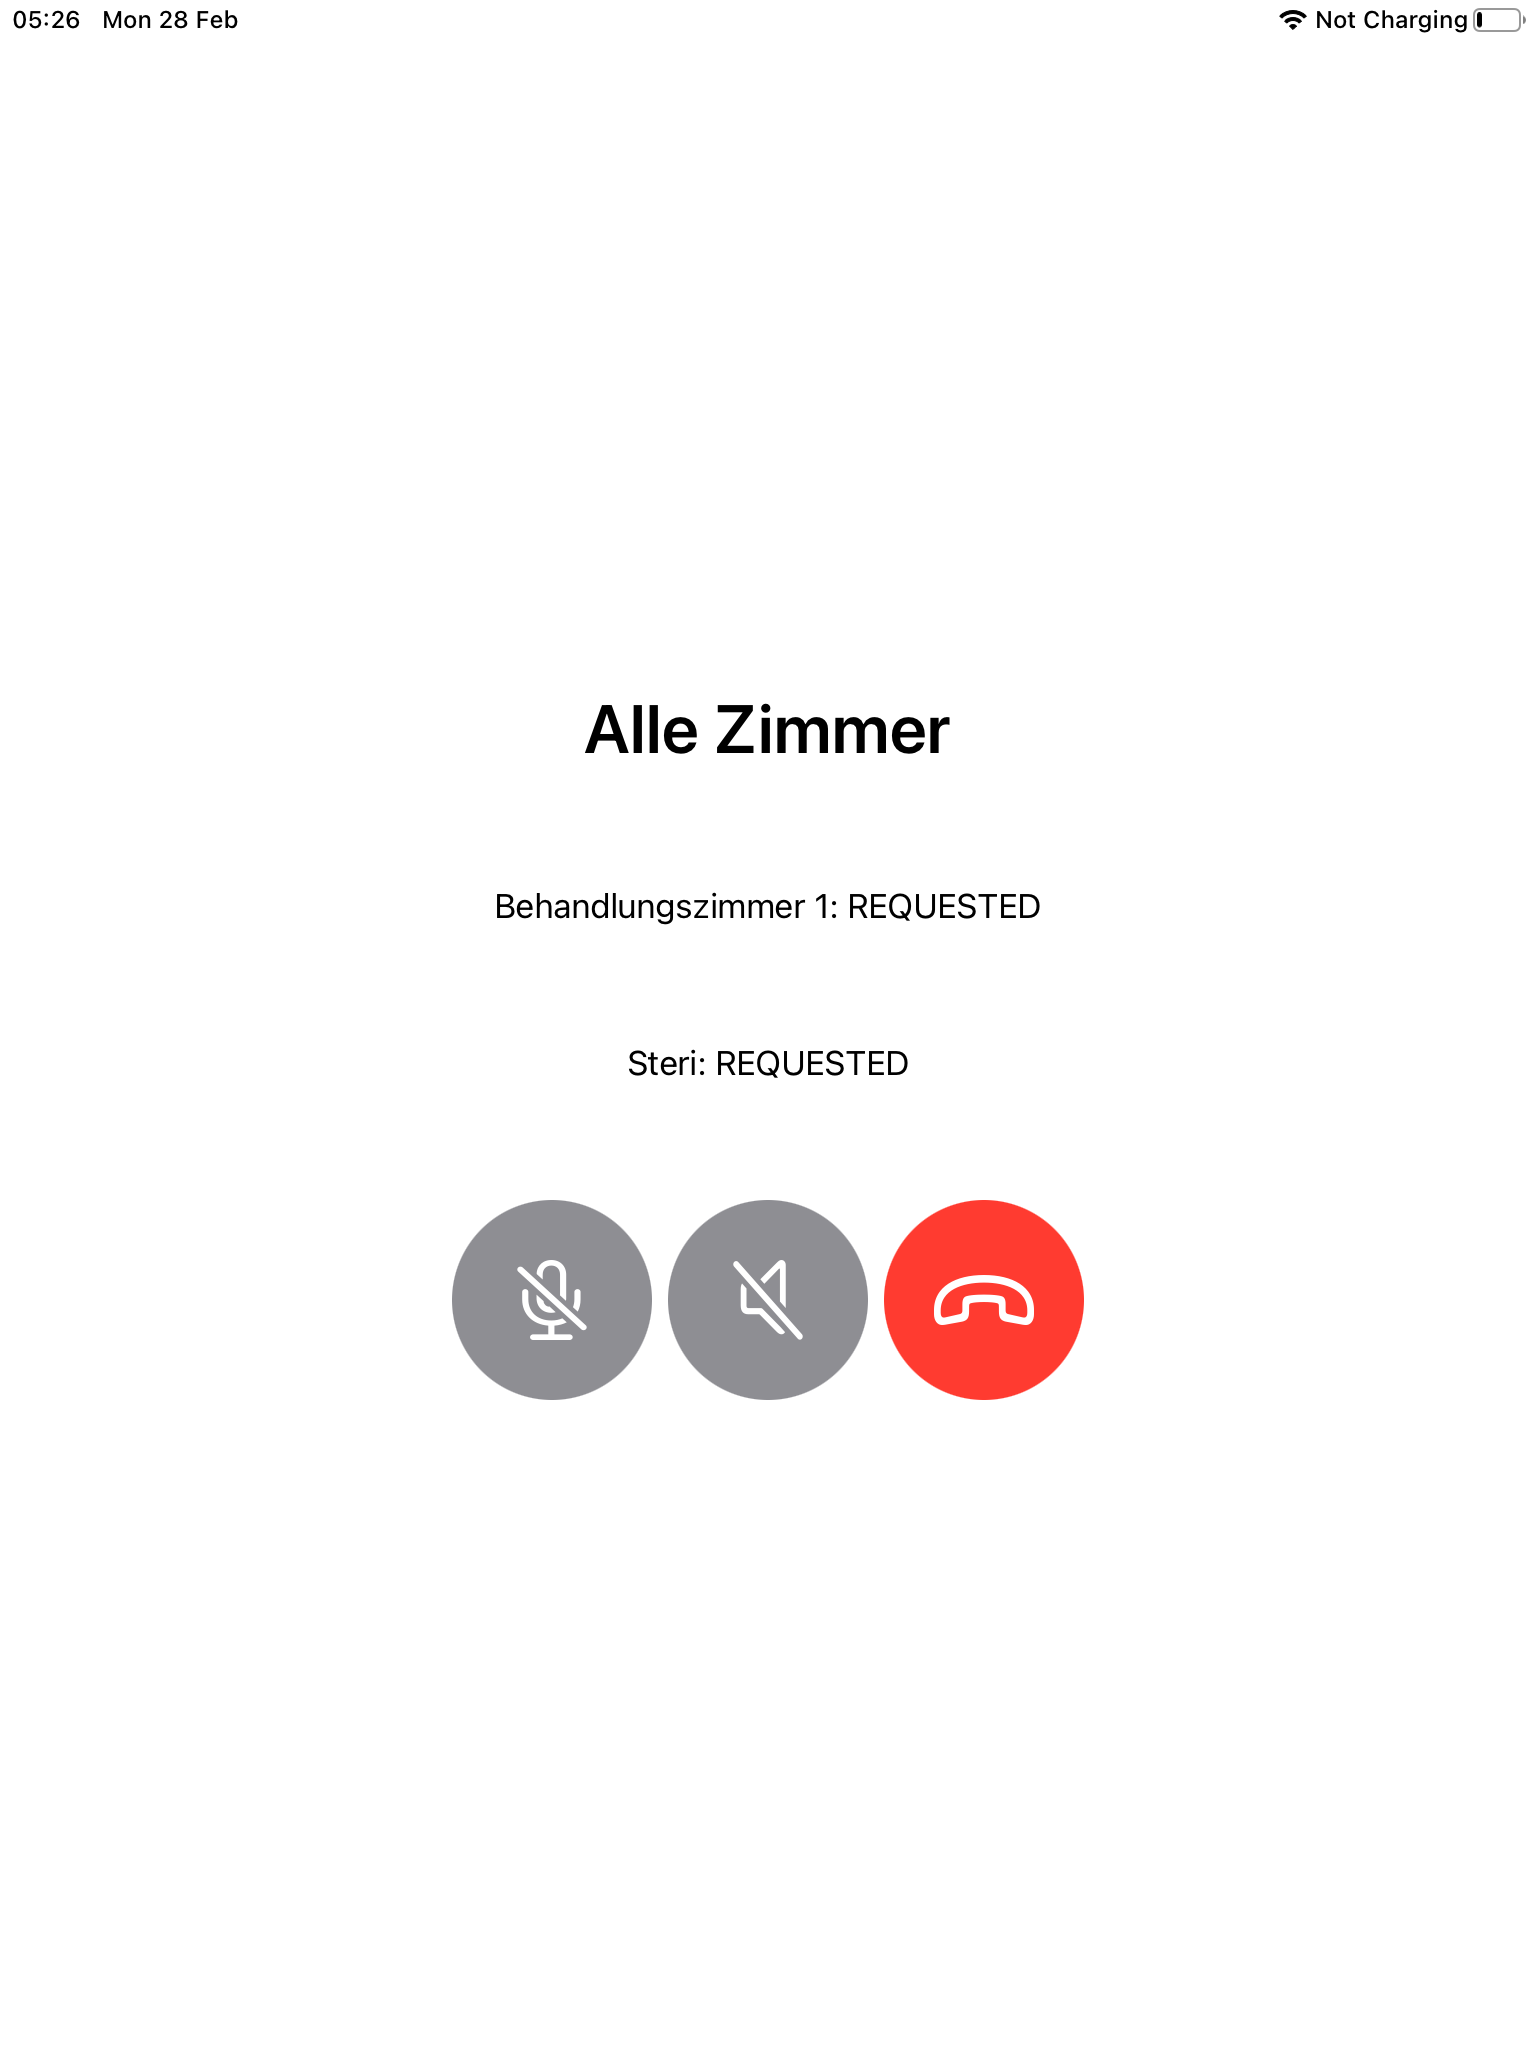
\includegraphics[width=\textwidth]{graphics/screenshots/app/call}}
        \caption{Ansicht Aktiver Anruf}
    \end{minipage}
    \label{fig:MobileClient-Screens3}
\end{figure}

Die Ansicht ''Aktive Anruf'' (Abbildung 8.6) wird angezeigt, nachdem ein Anruf gestartet wurde.
Entweder durch antippen eines Buttons in der Home Ansicht oder beim Empfang eines Anrufes von einem anderen Endgerät.
In dieser Ansicht wird der Titel des gestarteten Anrufes bzw.\ Name des Zimmer des Gesprächspartners angezeigt.
Wenn mehr als ein Gesprächspartner am Anruf beteiligt ist, wird zudem eine Liste der Teilnehmer zusammen mit deren Verbindungsstatus angezeigt.
Die Statusanzeige unterscheidet zwischen ''Verbindung erfolgreich'', ''Verbindung nicht erfolgreich'' und ''Verbindung in Arbeit''.
Allen Gesprächsteilnehmern stehen Buttons zur Stummschaltung des eigenen Lautsprechers und Mikrofons zur Verfügung.
Zudem können alle Gesprächsteilnehmenden die Unterhaltung durch den roten Auflegen Button beenden.

In Abbildung 8.6 wird ein Aktiver Anruf mit den Empfängern Empfang und Steri dargestellt.
Dabei hat die Verbindung zu Empfang den Status ''Verbindung hergestellt'' und die Verbindung zu Steri den Status ''Verbindung nicht erfolgreich''.
Konnte die Verbindung zu einem Empfänger nicht hergestellt werden, wird dieser mit einer Benachrichtigung darüber informiert.

\clearpage

\subsubsection*{Hintergrundbenachrichtigungen und Fehlerhandling}

Benachrichtigungen können mit Praxisruf auch empfangen werden, wenn die Praxisruf-App nicht aktiv ist.
Im Hintergrund empfangene Benachrichtigungen erscheinen als Push Benachrichtigungen auf dem Home Screen des iPads.
Anrufe über die Gegensprechanlage können nur empfangen werden, wenn die Applikation geöffnet ist.
Ist die App minimiert oder beendet, ist der jeweilige Client für Gespräche nicht verfügbar.
Ein nicht verfügbarer Client wird über Hintergrundbenachrichtigungen auf verpasste Anrufe hingewiesen.
Abbildung 8.7 zeigt eine Benachrichtigung ''Alarm'' und eine Benachrichtigung für einen Verpassten Anruf aus dem Zimmer Empfang.

\begin{figure}[h]
    \centering
    \begin{minipage}[b]{0.45\textwidth}
        \fbox{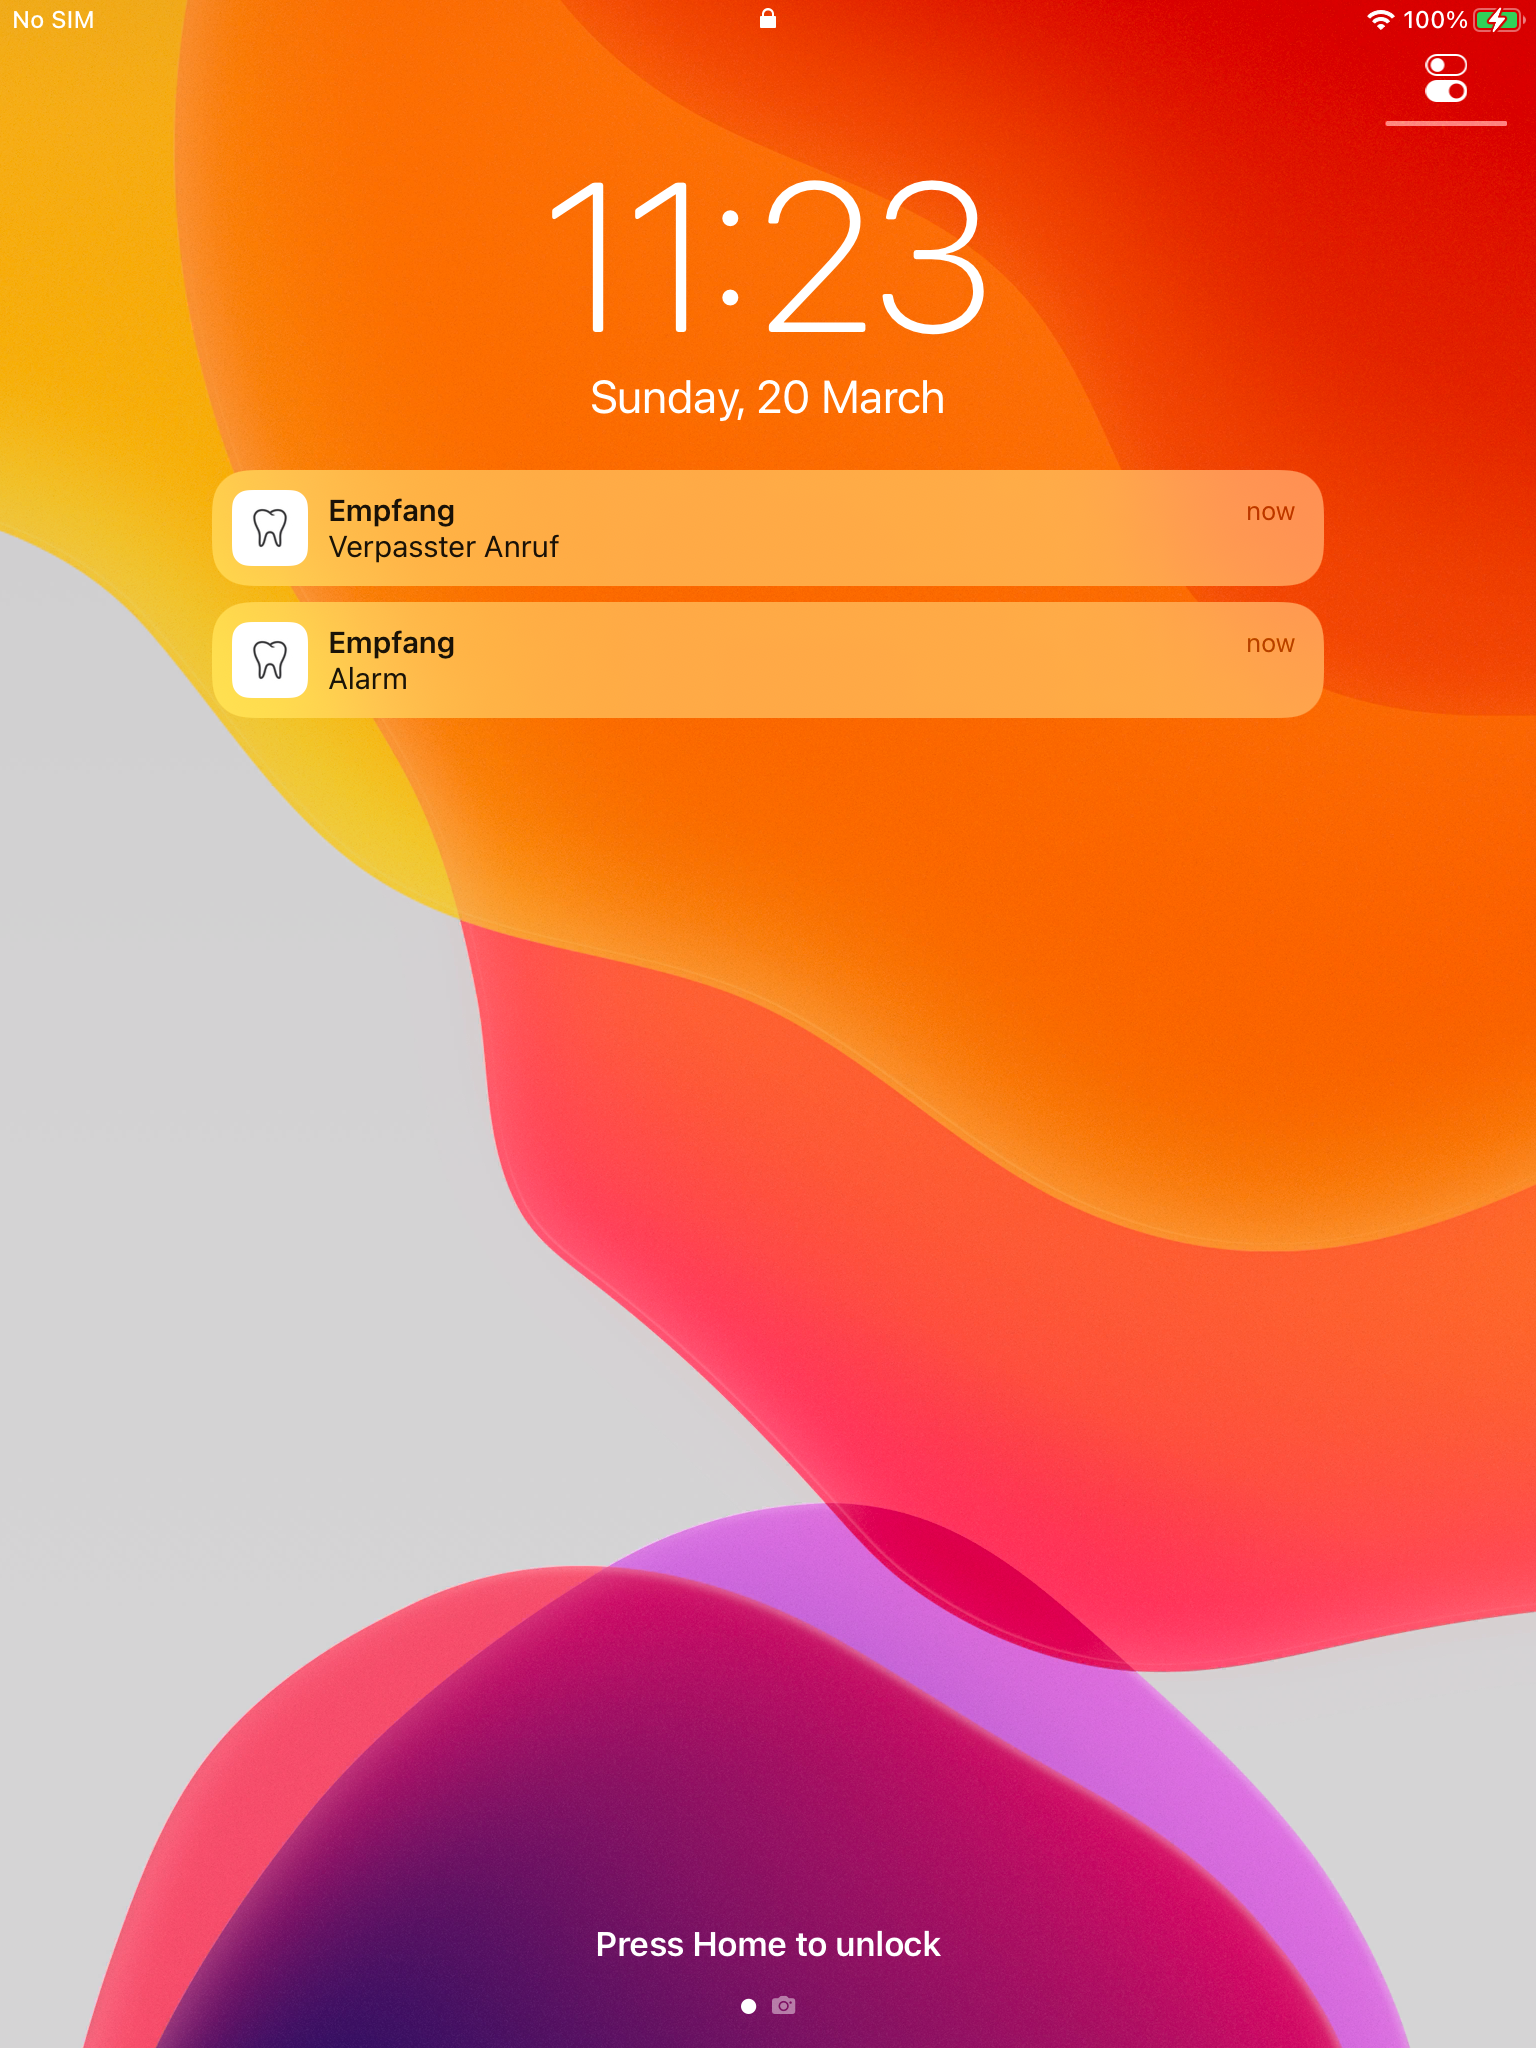
\includegraphics[width=\textwidth]{graphics/screenshots/app/background_notification}}
        \caption{Hintergrund Benachrichtigung}
    \end{minipage}
    \hfill
    \begin{minipage}[b]{0.45\textwidth}
        \fbox{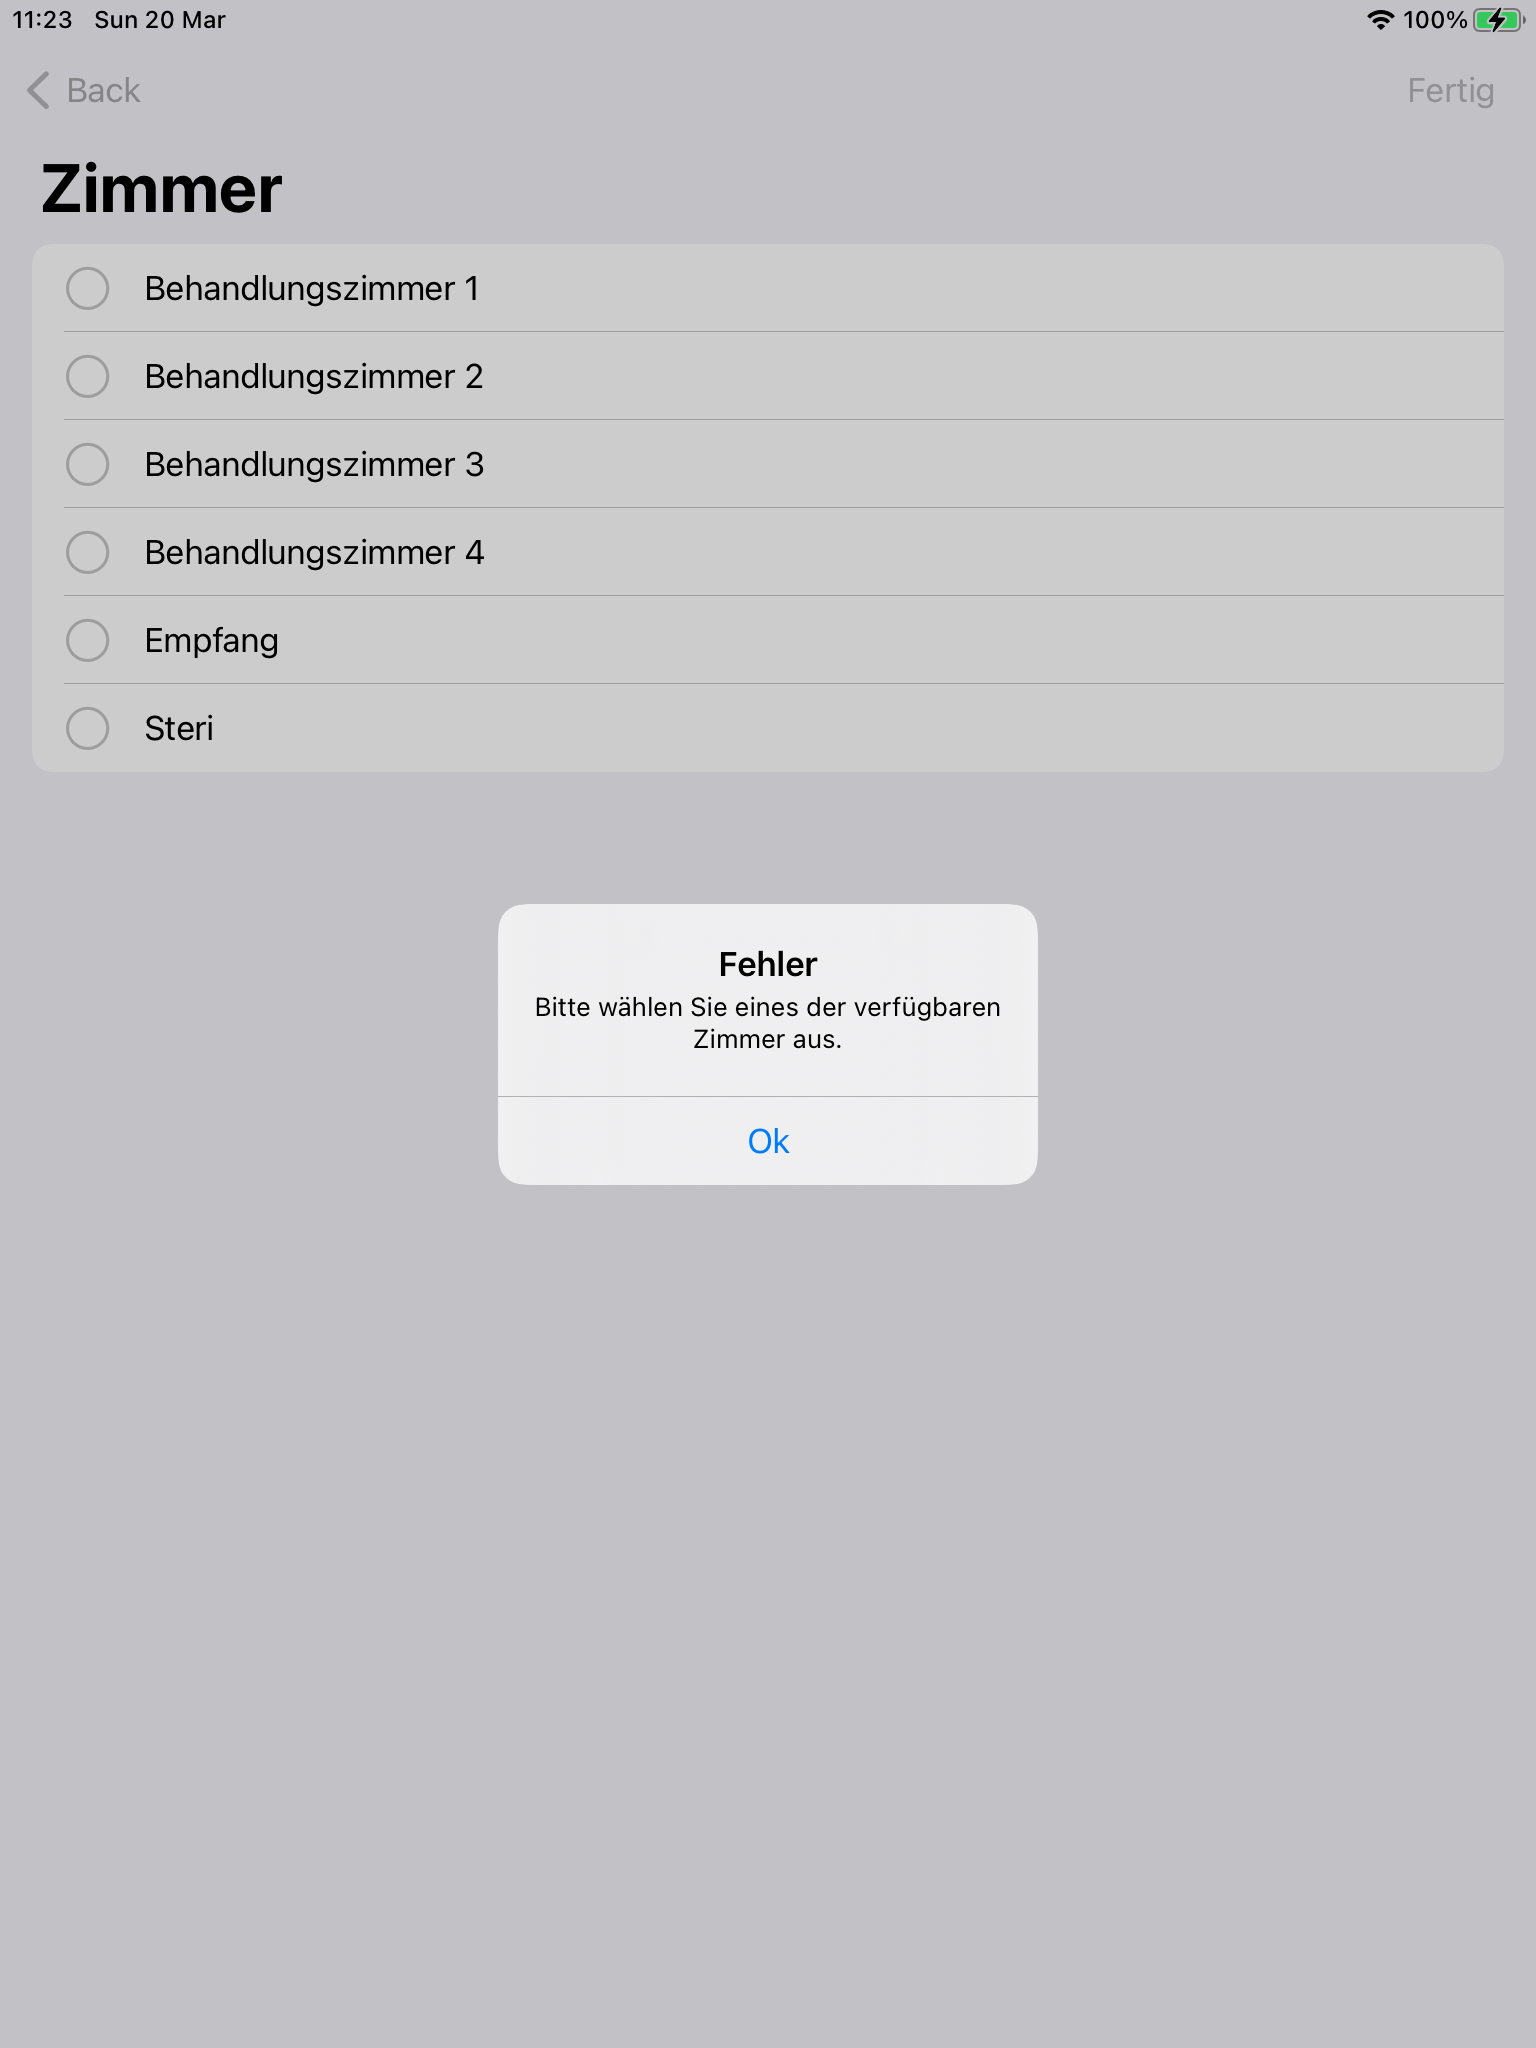
\includegraphics[width=\textwidth]{graphics/screenshots/app/error}}
        \caption{Ansicht Zimmerwahl - Fehlerdialog}
    \end{minipage}
    \label{fig:MobileClient-Screens4}
\end{figure}

Fehler in der Applikation werden dem Benutzer in einem einfachen Dialogfenster angezeigt.
Abbildung 8.8 zeigt eine Fehlermeldung, die bei der Auswahl der Zimmerkonfiguration auftreten kann.
Wenn die Wahl der Konfiguration bestätigt wird, ohne dass eine Konfiguration ausgewählt wurde, wird eine entsprechende Fehlermeldung angezeigt.

\clearpage


